\section{Design}

%以下两图展示了nfactor系统的基本架构。nfactor框架将统一的运行时系统组成cluster。在这个nfactor cluster内,细粒度的流管理可以被快速的执行。这个cluster由一个轻量级的控制器进行控制以实现动态扩展,和开启流迁移以及容错。

Figure \ref{fig:runtime} and \ref{fig:runtime-arch} daemonstrate the basic architecture of NFActor framework. NFActor framework composes uniform runtime systems into a cluster. Within this cluster, fine-grained flow managmeent tasks could be quickly executed. This cluster is controlled by a lightweight controller for dynamic scaling and inititiating flow management tasks, including flow migration and fault tolerance.

%nfactor的设计遵循了以下几个原则。
The design of NFActor framework follows the following principles.

\begin{itemize}

%第一,低开销。在提供复杂流管理的同时,nfactor也必须高速的处理数据包。因此,nfactor为每一个流所提供的execution context必须是一个轻量级的抽象,它不能对正常的NF处理产生比较大的性能影响。The execution context of nfactor framework是利用actor programming model 进行构建的。我们实现了自己的actor programming model库,从编程的角度考虑,消息传递的开销仅相当于一次函数调用。

\item \textbf{Low Overhead.} While providing compliated flow management tasks, the runtime system of NFActor framework must be able to process packets at high speed. Therefore, the execution context that NFActor created for each flow must be a lightweight abstraction, it should not compromise the processing speed of a NF. In NFActor, this execution context is constructed using actor programming model. We implement our own actor programming model to minimize the overhead associated with the execution context.

%第二,效率。 为了适应高速nfv系统的需求,nfactor所提供的流管理必须十分高效。在高速nfv系统中,一个NF每秒钟需要处理几百万个包,并控制几万流。在如此高速的吞吐量下实现流管理功能,这就要求nfactor避免使用内核网络协议栈,以避免上下文切换的的开销。在nfactor系统中,所有的数据处理,无论是dataplane的数据包还是actor发送的远程消息,都是利用高速的包IO (DPDK)来实现的。

\item \textbf{Efficiency.} To accomodate the need of high speed NFV systems, the flow management tasks of NFActor must be highlighy efficient. In high speed NFV systems, a NF may process millions of packets every second and handle tens of thousands of flows. To achieve high efficiency, NFActor completely abandoned using kernel networking stack to avoid the overhead of context switching. In NFActor, all the data, whethere it's data plane packet or remote actor messages, are transmitted through high-speed packet I/O (i.e. DPDK).

%第三,可扩展性。现代nfv系统必须具有良好的可扩展性,以适应不断变化的网络流量的需求。为了实现良好的可扩展性,nfactor系统提供了统一的运行时系统,并使用多个运行时系统组成nfactor cluster。在nfactor cluster内,运行时系统可以对经过自己的流进行路由管理,以实现动态的负载均衡。同时,我们也简单而快速的在不同的runtime之间传递信息,以实现高效的流管理任务。

\item \textbf{Scalability.} Modern NFV system must have good scalability, to accomodate varying network traffic. To provide good scalability, NFActor framework provides uniforms runtimes and connects multiple runtimes into a NFActor cluster. Within this cluster, the runtime system could manage output route for each flow that passes through it, to achieve dynamic load balancing. The uniform runtime design also faciliatates message passing among different runtimes, to achieve efficient flow management tasks.

\end{itemize}

\subsection{Runtime Cluster}


\begin{figure}[!t]
\begin{subfigure}[t]{0.30\linewidth}
   \centering
   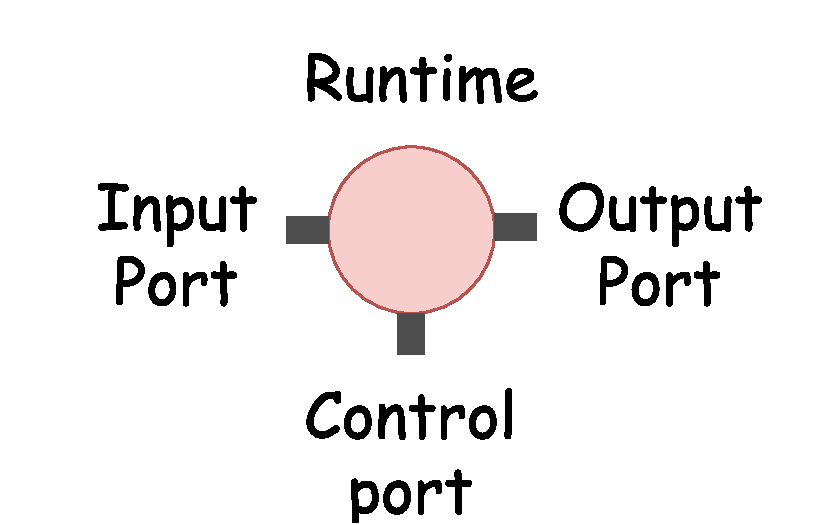
\includegraphics[width=\columnwidth]{figure/nfactor-runtime-with-port.pdf}
   \caption{A runtime with three ports.}\label{fig:runtime-with-port}
  \end{subfigure}\hfill
  \begin{subfigure}[t]{0.69\linewidth}
 \centering
   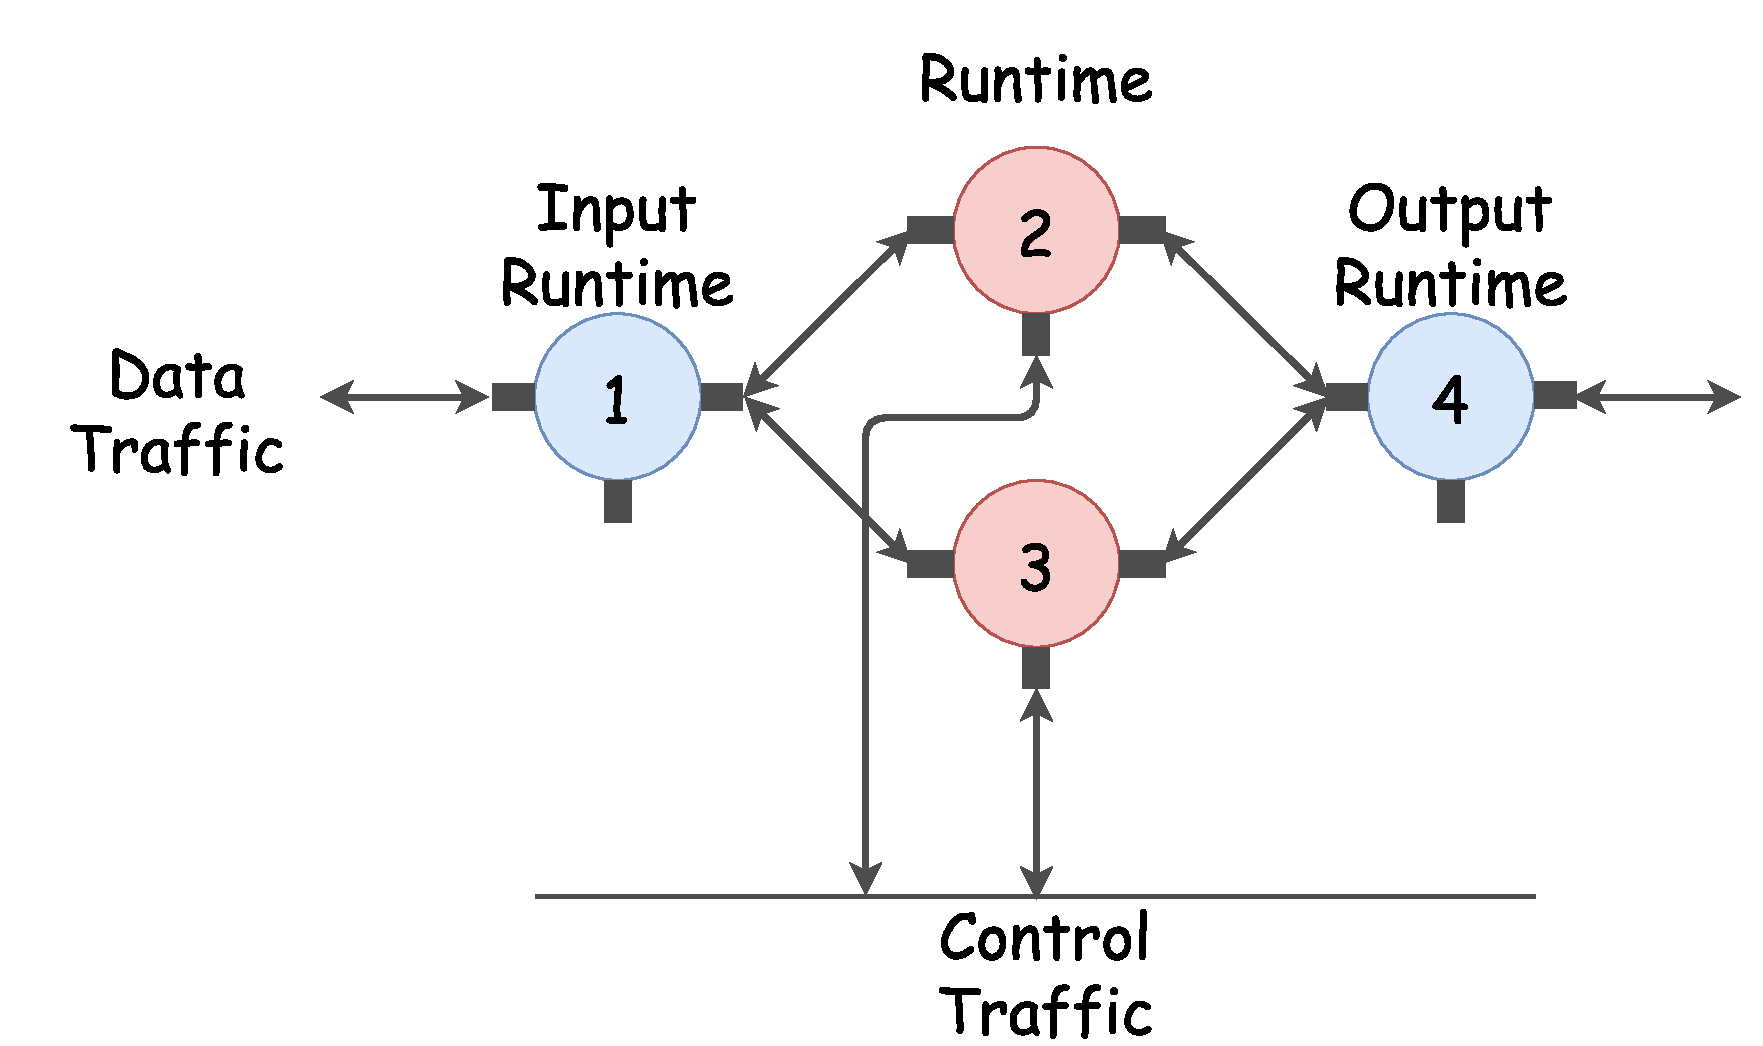
\includegraphics[width=\columnwidth]{figure/nfactor-runtime-connection.pdf}
   \caption{A minimal runtime connection.}\label{fig:runtime-with-io-runtime} \end{subfigure}\hfill
   \begin{subfigure}[t]{0.99\linewidth}
  \centering
    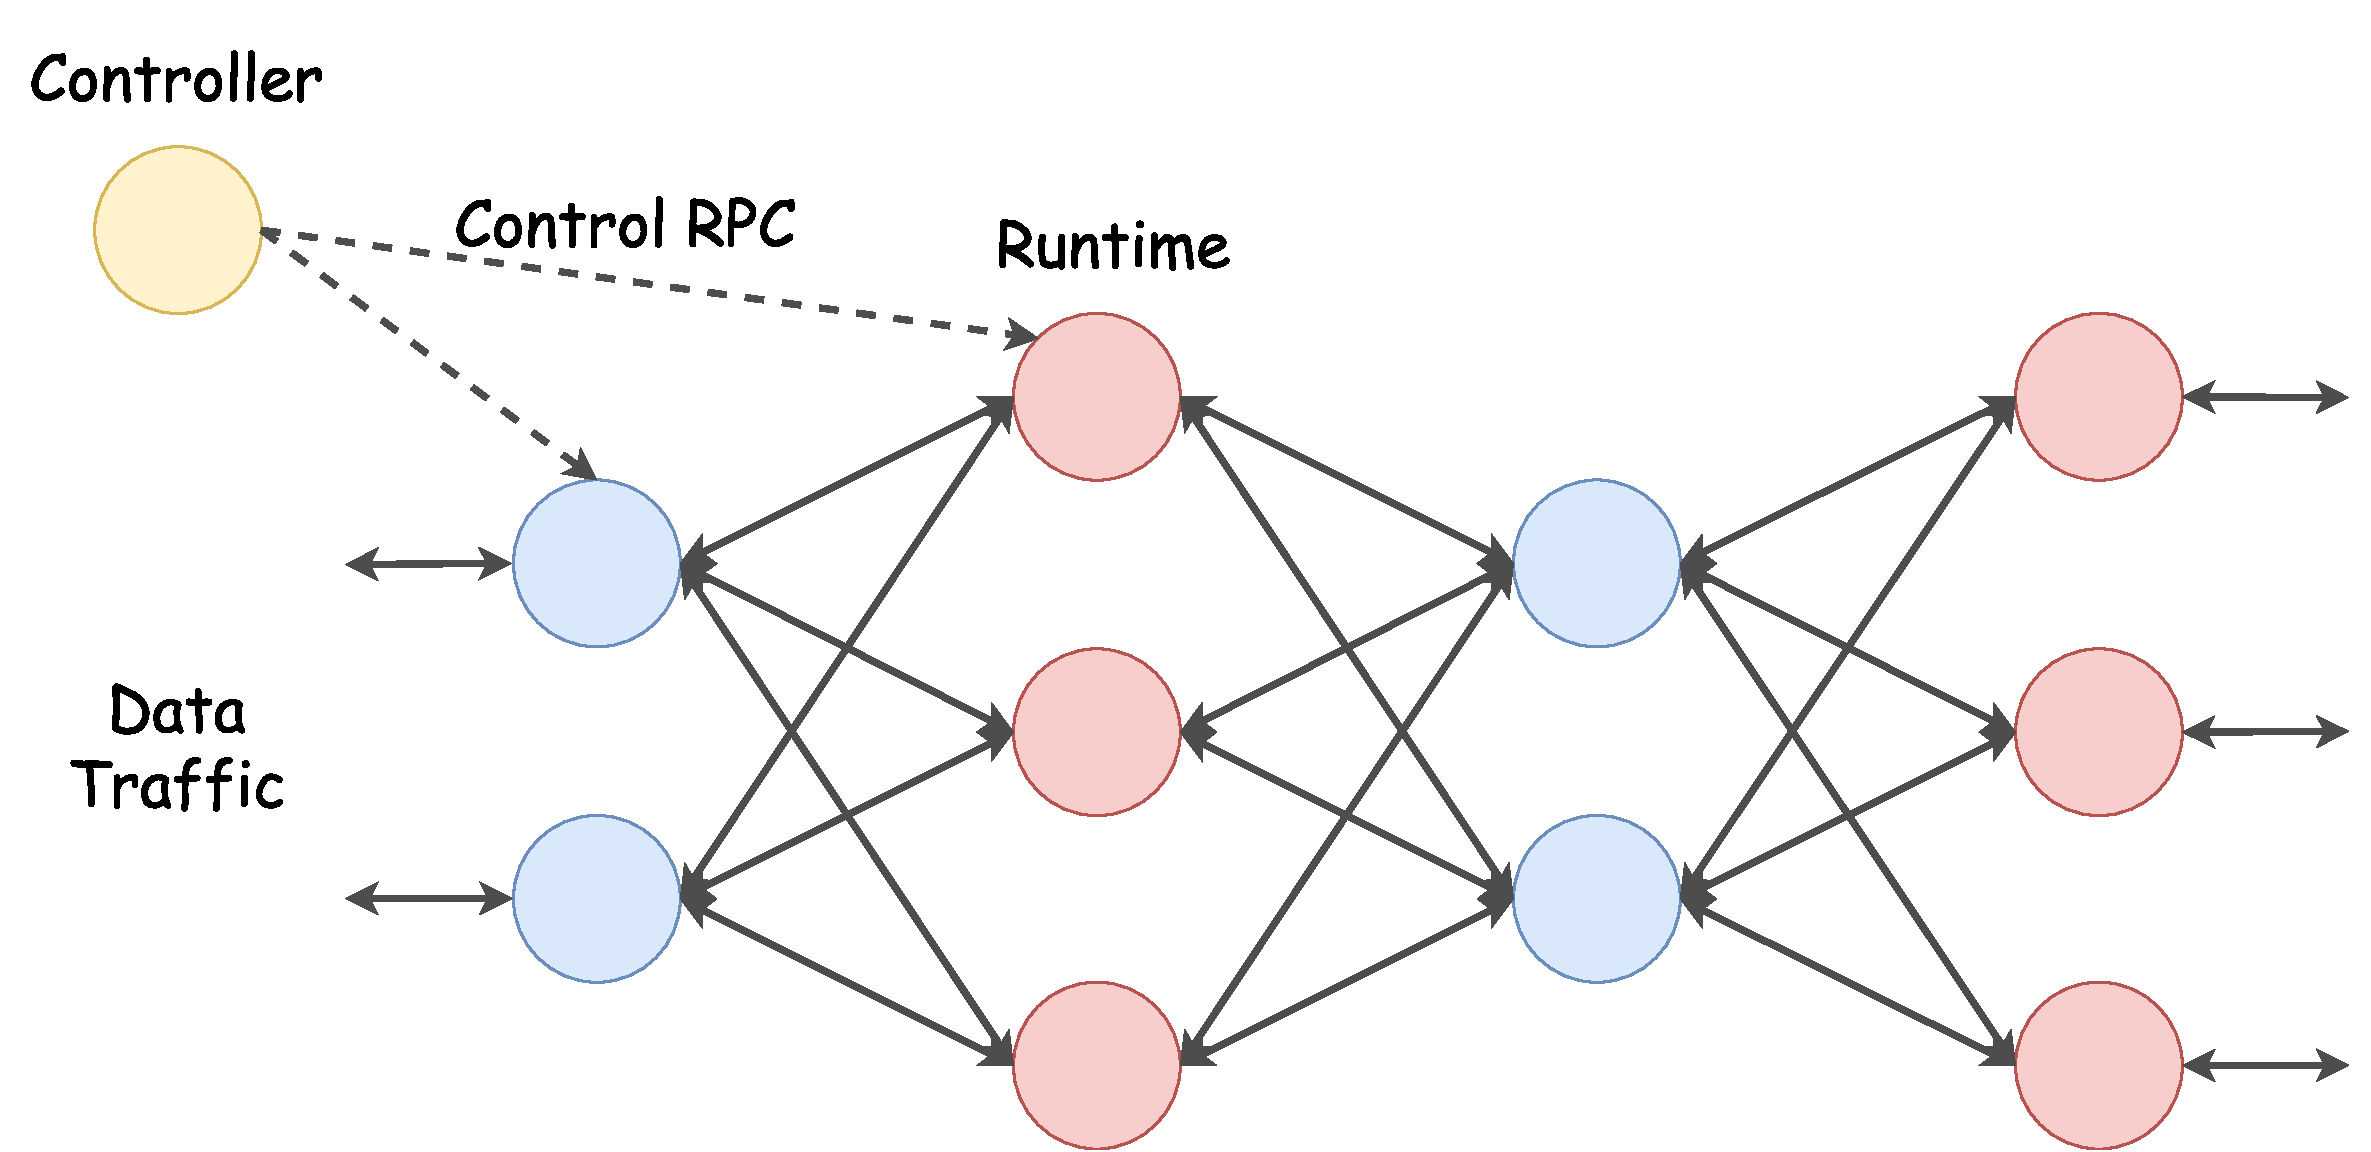
\includegraphics[width=\columnwidth]{figure/nfactor-cluster.pdf}
    \caption{A NFActor runtime cluster consists of multiple lay, controlled by a controller.}\label{fig:runtime-cluster} \end{subfigure}
 \caption{The flow migration performance of \nfactor}
\label{fig:runtime}
\end{figure}

%图1c展示了运行时cluster的基本结构。运行时cluster是由若干层运行时连接而成,并由一个轻量级的控制器利用RPC进行管理。
Figure \ref{fig:runtime-cluster} gives an example of a running NFActor cluster. The NFActor cluster consists of multiple runtimes controlled by a light-weight controller through RPC.

%图1a给出了一个runtime的基本结构。一个runtime包含三个端口。输入端口和输出端口用来接收和传递数据层的数据包。控制端口专门用来传递flow actor执行流管理任务时所生成的远程消息。输入输出端口也可以用来传递远程消息,我们在后面的章节中给出详细的解释。
Figure \ref{fig:runtime-with-port} shows the basic struture of a runtime. A runtime consists of three ports. The input and output ports are used to receive and send dataplane packets. The control port is only used to transmit remote messages when flow actor executes flow management tasks. Both input and output ports could also be used to transmit remote messages, this is further illustrated in later chapters.

%一个运行时系统自己并不能执行负载均衡以及流管理任务,它需要和其他的运行时系统进行连接才能完成这些功能。每一个运行时系统的三个端口都可以和其他多个运行是系统进行连接。图1b给出了一个能实现各种流管理功能的最小连接图。在图1b中,2号运行时系统的输入端口和输出端口分别与1号运行时系统的输出端口和4号运行时系统的输入端口相连,因此对于2号运行时系统而言,1号运行时系统时它的input runtime, 4号运行时系统时它的output runtime.同理,对于1号运行时系统而言,2号运行时系统时它的output runtime. 在NFActor framework中,运行时系统可以将自己的输出流量均匀分布在所有的输出运行时系统中。因此我们可以看到 dataplane traffic可以从图1b连接的一端进入并从另一端输出。

A runtime system could not execute any load-balacning and flow management tasks by itself. It needs to be connected with other runtimes and collaborate with those runtimes. The three ports of a single runtime system could be connected to multiple runtimes. Figure \ref{fig:runtime-with-io-runtime} gives a minimal runtime connection that is able to achieve load-balancing and flow management tasks. In figure \ref{fig:runtime-with-io-runtime}, the input and output ports of runtime 2 and 3 are connected with the output port of runtime 1 and input port of runtime 4. From the perspective of runtime 2, runtime 1 is its input runtime and runtime 4 is its output runtime. Similarly, runtime 2 is the output runtime of runtime 1. In NFActor framework, a runtime could balance its workload among all of its output runtimes. This is why the dataplane traffic could enter from one end of the connection in figure \ref{fig:runtime-with-io-runtime} and exit from the other end.

%对与2号和3号运行时系统而言,他们具有相同的input runtime和output runtime。我们将这一类运行时系统归纳入通一个layer。同一个layer的运行时系统的控制端口会被相互连接起来。同时,同一个layer的运行时系统之间可以实现快速高效的流迁移和容错。

From the perspective of runtime 2 and 3, they share the same input runtimes and output runtimes. These runtimes are classified into the same layer. The control ports of runtimes under the same layer are directly connected, so that flows could be quickly migrated and replicated among runtimes under the same layer.

%如图2所示,我们可以构建一个由multipile layers of runtime 所组成的nfactor cluster。这个cluster由一个轻量级的controller进行控制。controller可以检测每一个runtime的workload以实现动态扩展。同时,controller可以通过rpc来发起流管理任务的执行。

As shown in figure \ref{fig:runtime-cluster}, we can construct a NFActor cluster by creating multiple layers of runtimes. This runtime cluster could be controlled by a controller, which monitors the workload on each runtime for dynamic scaling. This controller could also initiate flow management tasks by sending RPC requests to selected runtimes.

\subsection{Runtime Architecture}

\begin{figure}
		\centering
		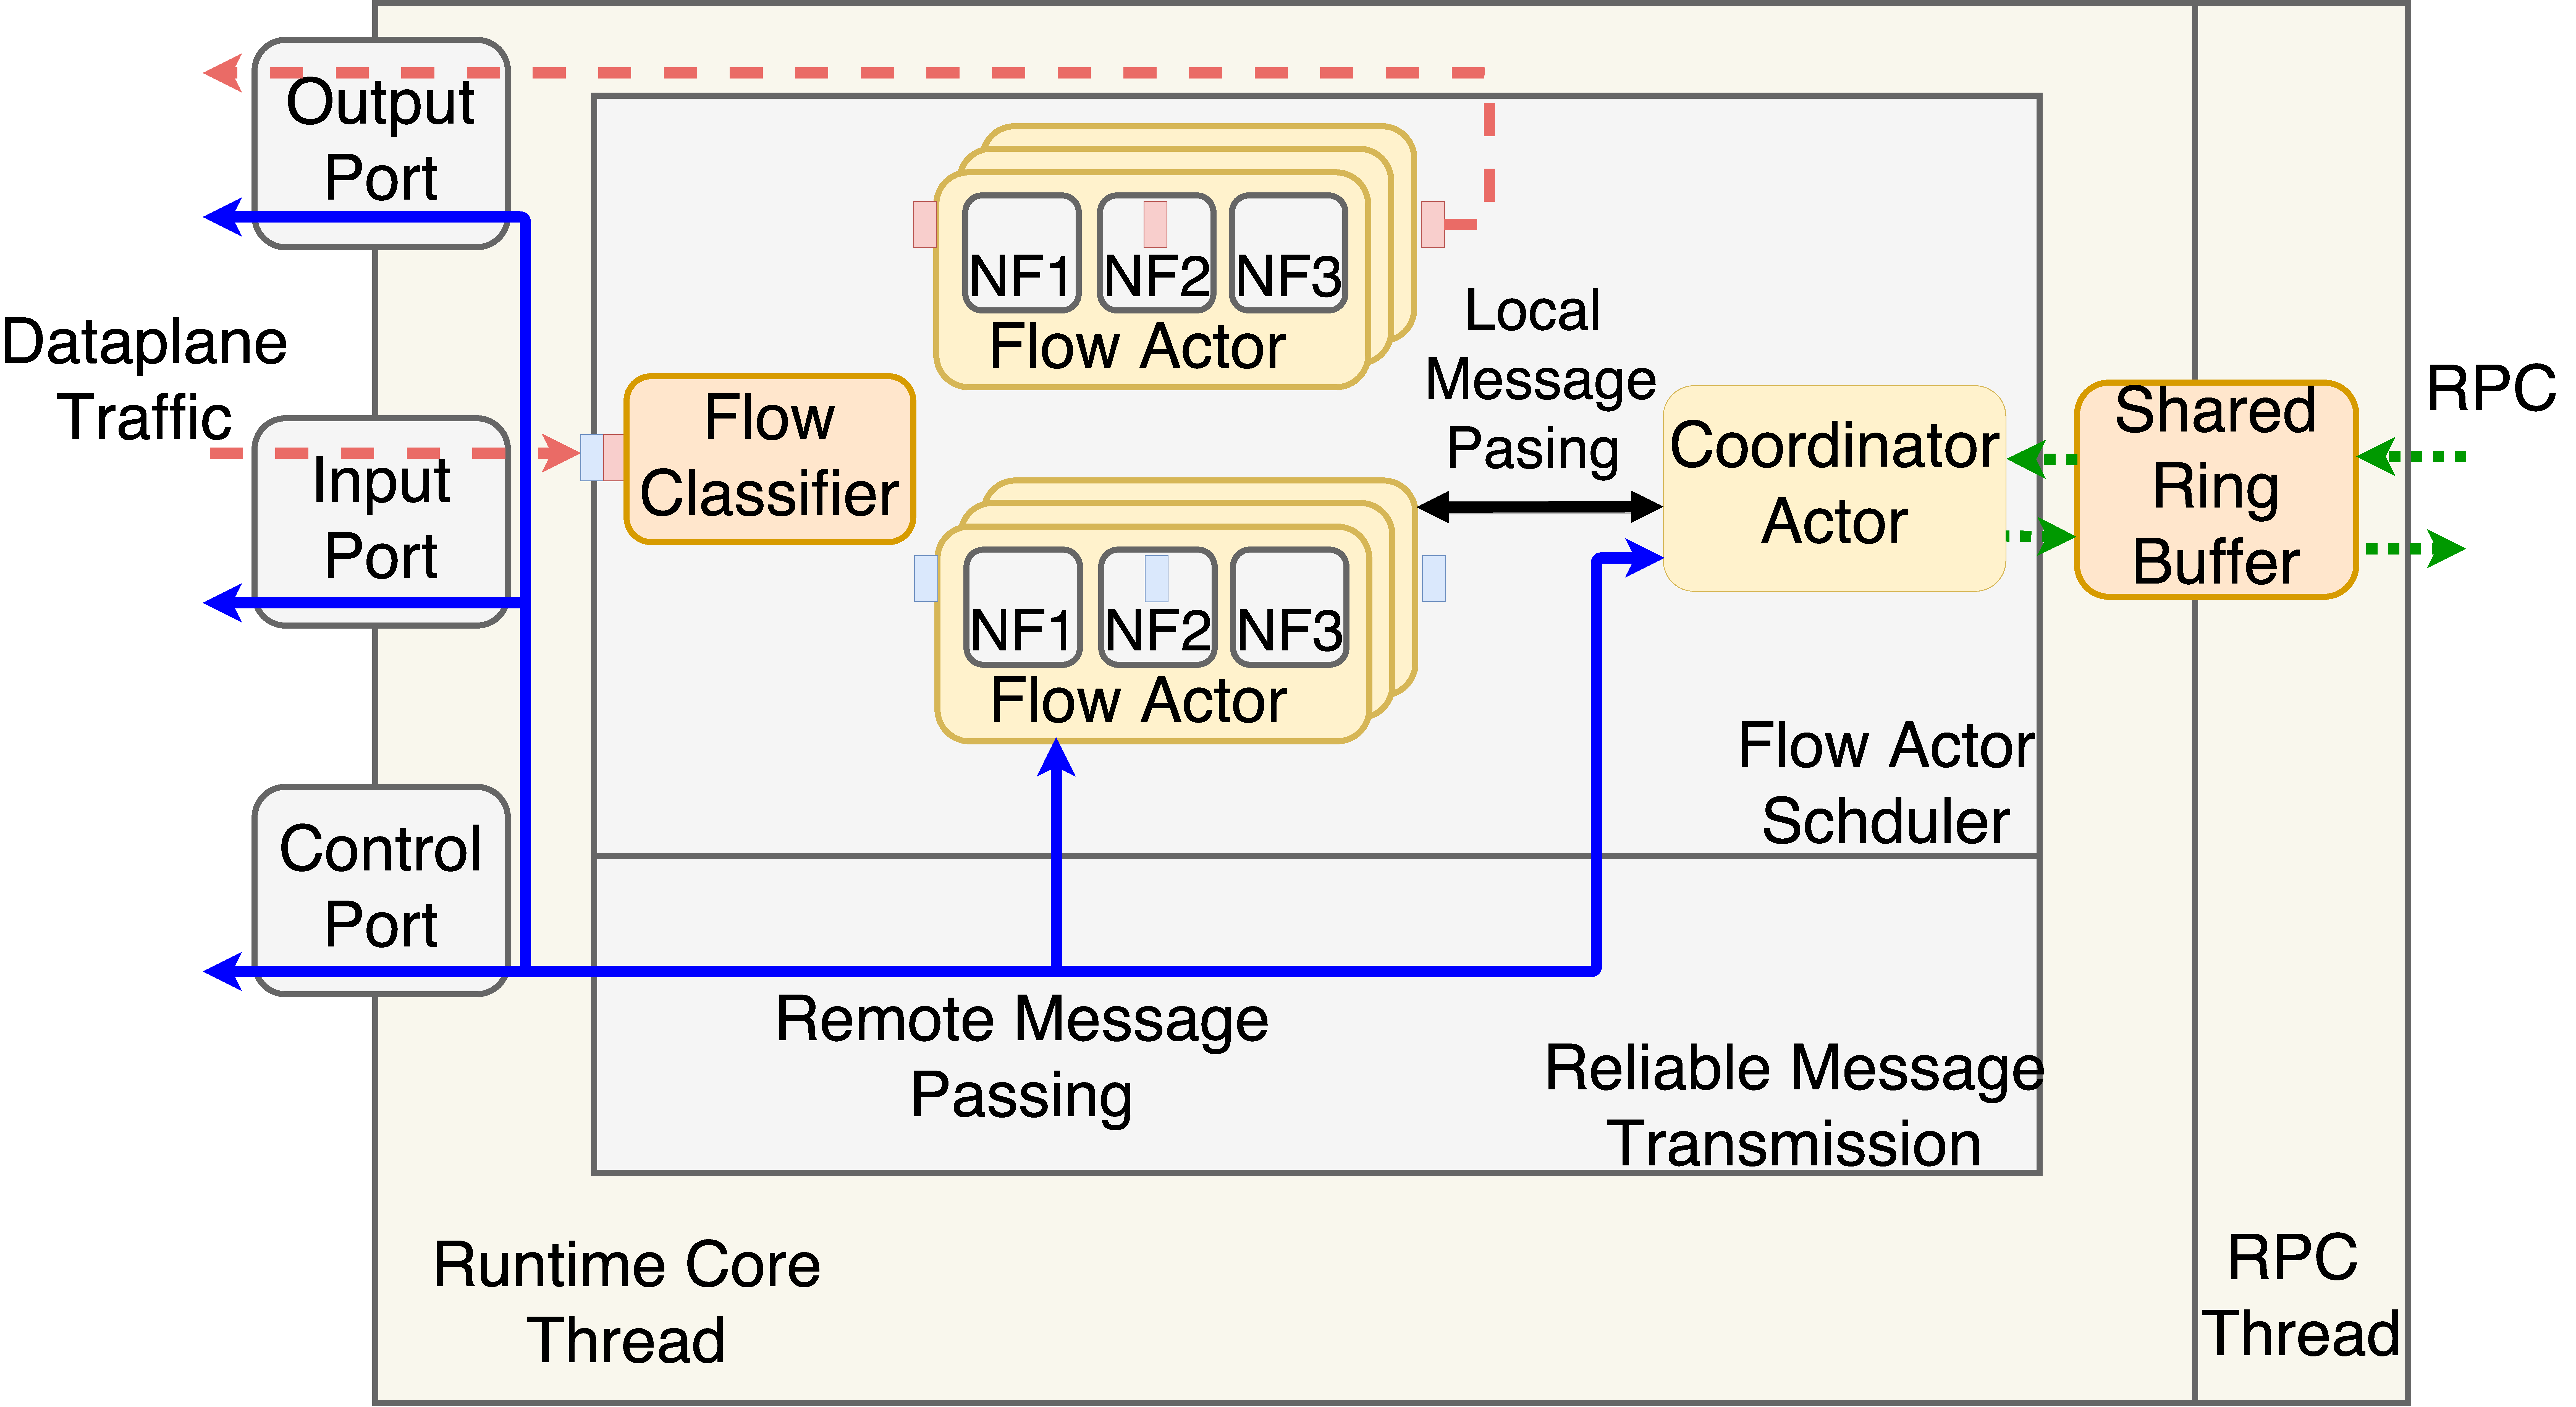
\includegraphics[width=\columnwidth]{figure/nfactor-runtime-arch.pdf}

		\caption{The internal architecture of a NFActor runtime system. }
\label{fig:runtime-arch}
\end{figure}

%图二展示了一个runtime的内部架构。一个runtime包含core thread 和rpc thread连个线程。rpc thread专门用来接收controller 发来的RPC 指令,并将这些指令利用一个共享的高速环形队列转发到core thread中。core thread里运行了两个重要的模块,分别是flow actor调度器和reliable message transmission module。这两个模块由一个模块调度器进行轮询调度。

Figure \ref{fig:runtime-arch} demonstrates the internal architecture of a runtime, which consists of an RPC thread and a core thread. The RPC thread receives RPC requests from the controller and forward these requests to the core thread using a shared ring buffer. The core thread has a flow actor scheduler module and a reliable message transmission module. Both of these two modules are scheduled to run by a round-rubin module scheduler. The core thread employs a run-to-completion scheduling model. The core thread keeps processing the input packet keeps processing until it is either dropped, or sent out from the output port.

%从输入端口获取的dataplane 的数据包会被直接发送给flow actor scheduler. flow actor scheduler 利用flow classifier对包进行分流。在我们当前的实现中,flow classifier使用传统的flow-5-tuple作为key来对包进行分流。flow classifier会为每一个新的流建立一个与之唯一对应的flow actor并将这个流的所有数据包交由flow actor进行处理。flow actor会将收到包依次通过一个在初始化时确定的service chain。当这个包完成处理时,flow actor会将这个数据包从输出端口送出。流调度器还会定时调度一个coordinator actor。这个coordinator actor负责从共享队列里提取rpc命令并执行rpc命令。

The core thread polls dataplane pacekts from the input port and forwards them to flow actor scheduler. The flow actor scheduler uses a flow classifier to classify packets into different flows. In our current implementation, the flow classifier uses tranditional flow-5-tuple (i.e. IP destination address, IP source address, transmission layer protocol, source port and destination port) to classify flows. Flow classifier creates an unique flow actor for each new flow, and forwards all the packets of a flow to its flow actor. The flow actor processes the packet by passing the packet through a pre-determined service chain at runtime initialization time. When the packet finishes processing, it is delivered to the output port. The flow actor scheduler also peoriodically schedules a coordinator actor, which is responsible for fetching RPC requests from the shared ring buffer and executes these requests.

% 同一个runtime上的flow actor和coordinator actor之间可以发送本地消息进行通信。不同runtime 上的actor可以利用reliable message transmission module来发送远程消息。在NFActor framework里,我们为每一个runtime分配一个唯一的runtime id,并为每一个actor分配一个唯一的actor id。 当进行远程actor message 传输时,发送actor只需要向reliable message transmission module指名接收actor 的id 以及接收actor所在的runtime id。消息就可以被可靠的传输出去。
Flow actor and coordinator actor on the same runtime could directly pass messages with each other. Actors on different runtime use reliable message transmission module to send remote messages. In NFActor framework, we assign a unique ID for each runtime and each actor. When an actor sends a remote message, it only needs to specify the actor ID of the receiver and the runtime ID of the receiver. The message is then delivered reliably to remote side by the reliable message passing module.


%一个runtime上只创建一个core thread的设计主要是为了减小使用actor programming model的overhead. 在我们最初的设计中,我们使用libcaf actor来构建flow actor。libcaf 库会建立自己的多个工作线程。flow actor会直接被这些工作线程进行调度。为了将从高速包IO端口获得包并发送给flwo actor,我们不得不再创建一个单独的轮询线程。在这种设计下,我们发现整个系统的最大吞吐量不会随着libcaf工作线程的增加而增大,因为前方的轮询线程会成为一个瓶颈。因此我们直接抛弃了多个工作线程的设计,采用一个core thread 来poll数据包,并调度flow actor。这种架构可以让我们对actor programming model采取很激进的优化,我们可以将消息传递通过函数调用进行直接实现,而不需要考虑同步问题。然后系统的scalability可以用过增加runtime的数目来实现。我们可以在evaluation章节中看到,这样的设计可以取得令人满意的效果。

The reason that a runtime has only one core thread is to improve resource utilization rate and minimize the overhead of using actor programming model. In our initial prototype implementation, we used LIBCAF \cite{caf} library to construct flow actors. LIBCAF library creates multiple worker threads and schedules flow actors to run onthese worker threads. In order to poll from the input port and send packet to flow actor, we have to create another polling thread. Under this design, we found out that the maximum throughput of a single runtime does not increase when the number of LIBCAF worker thread increases, because the polling thread has always been a bottleneck. Therefore, we abondan the multi-worker-thread design and use a single core thread to poll packets and schedule flow actors. This architecture allows us to perform aggressive optimization of actor programming model \ref{}. In the mean time, we can still maintain the scalability of the system by launching more runtimes. We show in evaluation section that this architecture could achieve satisfactory performance.

\subsection{Control RPCs}

%运行时系统暴露了一系列RPC以供controller进行调用。这些rpc可以分为以下几类:控制流管理任务的rpc仅仅
The runtime exposes a serise of RPCs for controller to use. A controller could use these RPCs to control the connection between different runtimes. In terms of flow management tasks, the controller only needs to participate in the initiation phase using the exposed RPCs. There's no need for the controller to get involved in the execution of flow management tasks, because flow actors could complete them by themselves. The controller using these RPCs could be designed as a light-weight one, this is a key difference that distinguish NFActor framework from previous work, where controller must be involved in each flow management task, thereby limiting the scalability of the system. These RPCs could be divided into the following categories.

\begin{itemize}

% 添加删除input/output runtime. 为一个runtime 添加或删除input/output runtime。当添加input/output runtime时,controller必须保证当前runtime的input port/output port与input/output runtime 直接相连。

\item \textbf{Adding Input(Output) Runtime.} This RPC call adds input(ouput) runtime to the RPC target(the runtime being called). Before calling this RPC, the controller must guarantee that the input(output) port of the RPC target is connected with the output(input) port of the input(output) runtime.

% 设置migration target。 为一个runtime设置migration target。migration target和当前runtime必须处于同一个layer。当设置好migration target后,controller可以发起另一个rpc,让当前runtime迁移多少流到migration target区。

\item \textbf{Migrating Flows to Migration Target Runtime.} This RPC call sets up a migration target runtime for the RPC target and indicates the number of flows to migrate. When this call finishes, the RPC target should start migrating flows to the migration target. The migration target must stay in the same layer as the RPC target.

% 设置replication target。 为一个runtime设置replication target。replication target和当前runtime也必须处于同一个layer。当设置好replication target后,新到来的流就会被replicate到replication target上。

\item \textbf{Setting up Repliation Target Runtime.} This RPC call sets up a replication target runtime. When this call finishes, the RPC target should start replicating new flows to the replication target runtime. The replication target must stay in the same layer as the RPC target.

% 恢复 failed runtime. 如果当前runtime 时failed runtime的replication target,那么保存在当前runtime上的flow replica就会被直接在当前runtime上恢复过来。
\item \textbf{Recovering Failed Runtime.} If the RPC target is the replication target runtime of the failed runtime, then flows replicated on the RPC target are directly recovered on the RPC target.

\end{itemize}

\subsection{NF Module}

%NFActor使用了模块化的NF设计。每一种NF都以一个模块的形式来进行实现,runtime系统可以加载并使用任何一种NF. 为了实现如图2中所示的service chain处理, 我们在runtime初始化时给它传递一个service chain的参数。在流处理过程中,runtime保证每一个flow actor都会将包依次经过service chain 所指定的NF。这个模块化的设计与Netbricks的模块系统比较相似。在 Netbricks,我们也可以在一个netbricks 运行时环境中加载多个NF并创建一个service chain。但是NFActor的NF module系统则为实现流管理功能作出了一定的设计上的改变。

Each NF used by NFActor is implemented as a loadable module. The runtime system could select which NF module to load and use. In order to achieve the service chain processing as indicated in figure \ref{fig:runtime-arch}, we pass in an argument indicating the composition of the service chain before initializing a runtime. The runtime guarantees that each flow actor processes the packet through each NF as indicated in the service chain. The modular NF design is similar to that in NetBricks \cite{199352}, however, NFActor modifies the interface exposed by the NF module to achieve efficient flow management.

%为了实现流管理,flow actor必须在任意时刻提取并封装当前的NF状态,并将这个流状态传递出去。为了快速的实现这一功能,我们将提议将NF的处理逻辑以及NF所保存的流状态进行完全的分离,并将NF所保存的流状态储存在flow actor内。每当flow actor处理包的时候, flow actor将当前的流状态和包一起传入NF处理逻辑中。 NF处理逻辑则直接对包和当前的流状态进行处理。我们在下表中总结了NFActor中构建NF module的API。可以看到,使用这组API,我们将NF module 转换成了一个基于流的有限状态机。这对于实现快速高效的流管理时十分有帮助的,当flow actor需要进行流迁移或容错的时候,它可以直接将自己当前的流状态传递出去,而不影响正常的NF处理。

When executing flow management tasks, flow actor must be able to extract and transmit the flow states of all the NFs on the service chain, without disturbing the normal service chain processing. To speed up this process, we propose to separate the flow state with the processing logic of the NF module, and store the flow state inside the flow actor.

We summarize the core APIs used by NFActor to construct new NF modules in figure \ref{fig:api}. Using these APIs, the flow actor could acquire a new flow state when it is created. When the flow actor processes a packet, the flow actor passes the current flow state and the input packet together into the processing logic of a NF module. The processing logic could directly update the flow state according to the input packet. Since the flow state is stored by the flow actor, the flow actor could directly manipulate its flow state when executing flow management tasks, without disturbing the NF processing logic.

\begin{figure}[!h]
\lstset{language=Python, showspaces=false,
        showstringspaces=false, tabsize=2, breaklines=true, basicstyle=\scriptsize,
}

\begin{verbatim}
  new_state = nf.acquire_new_flow_state()

  (output_pkt, updated_state) =
  nf.processing_logic(input_pkt, current_state)
\end{verbatim}

\caption{The core APIs used by NFActor to construct new NF modules.}
\label{fig:api}
\end{figure}

%当然,这样的设计也有一定的缺点,那就是比较难以实现共享状态的提取,转移和同步。但是,对于针对单一流而进行的流管理而言,保证共享状态的一致性是一件非常困难的事情。这个过程中可能需要多层的同步,从而影响单个流管理任务的处理速度。在设计NFActor的时候,我们主要的目标是为单个流的管理提供一个高效的运行环境,因此我们并没有考虑对共享状态进行同步。Instead,当流管理对某个NF共享状态的一致性产生影响时,我们可以给NF提供一个函数,以显示的通知NF流管理通知所造成的影响。

Even though this design facilitates flow management tasks, it has its own limitation. Using this design, it is hard to extract and tranismit shared states. However, it is a complicated tasks to guaratee the consistency of shared states when managing a single flow. It may require multiple synchronizations, thereby affecting the processing speed of a single flow management task. Sice our primary goal when designing NFActor is to provide a high performance exeuction context, we do not aim to synchronize shared state. Instead, when flow management affects the consistency of the shared state, we could explicitly notify the NF about the result of flow management tasks and let NF module to handle the inconsistecy.



\subsection{Route Selection}

%在nfactor cluster中,由于有多层runtime的存在,因此我们需要为每一个flow进行路由选择。这个功能被直接赋予每一个 flow actor。当一个新的flow actor被创建时,flow actor会在使用轮询的方法在所有的output runtimes里选择一个来当作自己的目的地runtime。当flow actor处理完一个输入包后,它会将包的目的地改为目的地runtime的input port 的mac地址,并将包的源mac地址改为自己input port的mac地址,并将包送出去。flow actor也会分析引发flow actor创建的包的源mac地址,以确定这个流是从哪个runtime发送过来的。

In a NFActor cluster, the existence of multiple layers of runtimes require us to do route selection for each flow. This functionality is directly assigned to each flow actor on the runtime. When a new flow actor is created, the flow actor select an output runtime as its destination using round-rubin algorithm. Before flow actor sends an input packet out, it replaces the destination MAC address of the packet with the MAC address of the input port of the destination runtime, and modifies the source MAC address as the MAC address of the output port of the current runtime. The flow actor also analyzes the source MAC address of the input packet to determine which input runtime the flow comes from.

We can see from later section that, when executing flow management tasks, the route of the flow needs to be dynamically changed. Since each flow actor has route selection functionality, the flow actor could directly send messages to the flow actors on its previous hop and next hop to modify the route.

%在后面的章节中我们可以看到,当执行流管理任务时,我们需要动态的改变改变流的路由。由于每一个flow actor都具有路由选择功能,因此flow actor可以直接向自己的上一跳flow actor和下一跳的flow actor发送改变路由的消息来改变路由。


\subsection{Flow Management}

%在这一章中我们介绍NFActor的流管理功能。在NFActor中,每一个flow的管理任务都是由相对应的flow actor自主执行的,这使得流管理并不需要一个中央管理器进行直接协调,提供了前所未有的scalability。同时,因为在nfactor cluster中,每一个流可以自己进行路径选择,因此nfactor的流管理完全不需要借助sdn,这显著提高了流管理执行的速度。最后,在nfactor 所使用的nf module实现了完全的流状态和nf处理逻辑的分离,flow actor可以在任意时刻直接对流状态进行操作,因此整个流管理的过程对nf来说时完全透明的。任何利用nf actor所提供的接口实现的nf module都可以和流处理功能进行无缝衔接。对于programmer而言,这使得他们在实现nf module时可以集中与nf内部的逻辑设计,而不需要考虑怎样和流管理进行融合。这大大提高了流管理的易用性。

In NFActor, the flow management task is automatically executed by each flow actor, without the coordinator from a central controller. This feature provides good scalability when there are multiple runtimes in the cluster. Inside a NFActor cluster, each flow could do route selection by itself, therefore there is no need to rely on SDN switches and controllers. This improve the usablility and performance of NFActor framework, because SDN may not be available at all time and SDN incurs a high processing overhead when dynamically changing flow rules. Finally, the new NF modules APIs completely separate the flow state with NF processing logic. The flow actor could manipulate the flow states at any time, and the entire flow management tasks are completely transparent to the NFs. Any NF modules implemented on top of the APIs provided by NFActor could be seamlessly integrated with flow management tasks. From the perspective of NF module programmers, this feature helps them focus on the internal logic design when implementing NFs, instead of considering how to integrate their code with complicated flow management tasks. This greatly impiroves the applicability of NFActor framework. The following 2 sections give details about how flow migration and replication tasks are implemented in NFActor system.

\subsubsection{Flow Migration}
%如图中所示,当flow actor收到migrate to migration target runtime的命令后,它开始进行migration。migration包含了以下三组request-response。
As is shown in figure \ref{}, when the current flow actor being migrated receives a migration command, it starts flow migration by executing the following three groups of request-responses.

\begin{itemize}

%第一,flow actor会向migration target runtime的coordinator发送一个请求,这个请求中含有当前flow actor的flow-5-tuple。coordinator接收到这个请求后使用包含在请求中的flow-5-tuple来创建一个migration target actor。这个migration target actor在migration完成后就会代替当前flow actor的身份。当migration target actor建立完成后,它会向当前flow actor给出一个response。

\item \textbf{First,} the current flow actor sends a request to the coordinator actor on the migration target runtime, containing the flow-5-tuple of the current flow actor. After receiving this request, the coordinator actor creates a migration target actor using the flow-5-tuple contained in the request. The migration taget actor then gives a response to the current flow actor.

%第二,flow actor会向它的上一跳input runtime的coordinator actor发送一个请求,这个请求也携带了flow actor的flow-5-tuple和migration target runtime的id。coordinator actor则利用flow-5-tuple找到上一跳flow actor,并通知上一跳flow actor将它的输出路径修改为migration target runtime。当路径修改完成以后,上一跳flow actor会给当前flow actor一个response。当路径修改完成以后,migration taget就会开始接收到数据包,它会将收到的数据包保存到一个buffer内知道第三组request-response完成。

\item \textbf{Second,} the current flow actor sends another request to the coordinator actor of its previous hop runtime, containing the flow-5-tuple and the ID of the migration target runtime. The coordinator actor uses the flow-5-tuple to find out the flow actor on the previous hop and notifies that flow actor to modify its output route to the migration target runtime. When the flow actor on previous hop finishes modifying the route, it gives a response back to the current flow actor. Also, after route modification, the migration target starts to receive data packets. The migration target actor buffers the data packets until the third group of request-response finishes.

%第三,flow actor将自己的flow state 作为消息传递给migration target actor。migration target actor收到flow state后,将flow state保存起来,给出回复并立刻对所有的buffer packets进行处理。current flow actor则在接收到回复后退出。

\item \textbf{Third,} the flow actor sends its flow state to the migration target actor. After receiving the flow states, the migration target actor saves them, gives a response to the current flow actor and immediately start processing all the buffered packets. The current flow actor exits when receiving the response.

\end{itemize}

\textbf{Lossless Migration.} Even though the three request-responses are seemingly trivial, they actually achieve lossless migration as defined in OpenNF. If the three request-responses are successfully completed, the flow being migrated will not miss processing a single packet. The key reason is that when the flow actor being migrated receives the second response, it will not receive any more data plane packet sent to it anymore. This is because the second response is actually delivered by the same network path as the data plane packets. Recall that in figure \ref{fig:runtime-arch}, the remote messages could also be sent over input/output ports of a runtime. The second response is actually sent by the output port of the previous hop runtime and received by the input port of the current runtime, thereby sharing the same network path as the data plane packets. If the network does not re-order any packets (the network could indeed re-order packets, but the possibility is extremely low and there is no known method to fight agaist this kind of error) , then the current flow actor receives no more dataplane packets because the route has been changed prior to the previous hop actor sending out the second response. Therefore, no packet is missed during the migration operation.

\textbf{Error Handling.} The three request-responses may not always be successfully executed. In case of request failure, the current flow actor is responsible for restoring the modified route (if it happens) and resumes normal packet processing. The migration target actor is deleted after a timeout.



\subsubsection{Flow Replication}

\subsection{Dynamic Scaling}
